\documentclass[aps,onecolumn,11pt]{revtex4}
\usepackage{graphicx}
\usepackage{amssymb,amsfonts,amsmath,amsthm}
\usepackage{chemarr}
\usepackage{bm}
\usepackage{pslatex}
\usepackage{xfrac}
\usepackage[dvipsnames]{xcolor}
\usepackage{bookman}
\usepackage{dsfont}
%\usepackage{mathptmx}
%\usepackage{hyperref}
%\usepackage{rotating}
\usepackage{fancybox}

\newcommand{\mychem}[1]{\mathtt{#1}}
\newcommand{\myconc}[1]{\big[#1\big]}

\newcommand{\Faraday}{\mathrm{F}}
\newcommand{\spx}{\mychem{X}}
\newcommand{\spLi}[1]{{\!~^{#1}\mychem{Li}}}
\newcommand{\Li}[1]{\myconc{\spLi{#1}}}
\newcommand{\spproton}{\mychem{H}}
\newcommand{\proton}{\myconc{\spproton}}

\newcommand{\myleak}[1]{\left.{#1}\right\vert_{\mathrm{leak}}}
\newcommand{\myout}[1]{{#1}_{\mathrm{out}}}
\newcommand{\LiOut}[1]{\myout{\Li{#1}}}
\newcommand{\spLiOut}[1]{\myout{\spLi{#1}}}

\newcommand{\myrotate}[2]{\rotatebox[origin=c]{#1}{#2}}

\newcommand{\mytrn}[1]{{#1}^{\!\mathsf{T}}}
\newcommand{\mymat}[1]{{\bm{#1}}}
\newcommand{\mydet}[1]{{\left|{#1}\right|}}

\usepackage{ifthen}


\newcommand{\LiAll}{\Lambda}
\newcommand{\LiAllOut}{\myout{\LiAll}}
\newcommand{\inpLi}[1]{\text{+}\spLiOut{#1}}
\newcommand{\outLi}[1]{\text{-}\spLiOut{#1}}

\newcommand{\mycolor}[2]{\ifthenelse{\equal{#1}{6}}{{\color{Red}#2}}{{\color{Green}#2}}}



\begin{document}
\title{Cooperativity}
\maketitle
%\tableofcontents

\section{Passive Behaviour}
We have two species $\spLi{6}$ and $\spLi{7}$ that may leak through the membrane:
\begin{equation}
	\partial_t \myleak{\Li{u}} = k_u \left( e^{\dfrac{-\Faraday V_m }{RT}} \LiOut{u} - \Li{u}\right)
\end{equation}

\section{One Layer}

\subsection{Scheme}
{
\Large
\begin{equation}
\boxed{
\begin{array}{ccccc}
 & & E_{06}  &  & \\
 &  \mycolor{6}{\myrotate{45}{$\xrightleftharpoons[\outLi{6},\;d_{06}]{+\spLiOut{6},\;a_{06}}$}} &   & \mycolor{6}{\myrotate{-45}{$\xrightarrow[-\spLi{6}]{+ \spproton, \; k^p_6}$}} &  \\
E_{00}  &  & \xleftarrow{\text{ recycling } k_h } &   & E_{0H} \\
  & \mycolor{7}{\myrotate{-45}{$\xrightleftharpoons[\outLi{7},\;d_{07}]{+\spLiOut{7},\;a_{02}}$}} &   & \mycolor{7}{\myrotate{+45}{$\xrightarrow[-\spLi{7}]{+ \spproton, \; k^p_7}$}} & \\
 & & E_{07} & & \\
 \end{array}
 }
\end{equation}
}

\subsection{Equations}

\begin{equation}
\left\lbrace
\begin{array}{rcl}
\partial_t E_{00} & = & D_{06}-A_{06} + D_{07}-A_{07} + v_h\\
\partial_t E_{06} & = & -D_{06}+A_{06} -v^p_6 \\
\partial_t E_{07} & = & -D_{07}+A_{07} -v^p_7\\
\partial_t E_{0H} & = & v^p_6 + v^p_7 - v_h\\
\mathsf{E}       & = & E_{00}+E_{01}+E_{02} + E_{0H} = E_{0H} + {\displaystyle \sum_{x\leq y\leq 1} E_{xy}}\\
\end{array}
\right.
\end{equation}
with
\begin{equation}
\left\lbrace
\begin{array}{rcl}
A_{06} &= &a_{06} E_{00} \LiOut{6}\\
A_{07} &= &a_{07} E_{00} \LiOut{7}\\
D_{06} &= &d_{06} E_{06}\\
D_{07} &= &d_{07} E_{07}\\
v^p_6  &=& k^p_6 E_{06} \proton\\
v^p_7  &=& k^p_7 E_{07} \proton\\
v_h    &=& k_h   E_{0H}
\end{array}
\right.
\end{equation}

\subsection{Steady-State}
\subsubsection{Raw Equations}
We assume that the internal components are at a steady-state:
\begin{equation}
\left\lbrace
\begin{array}{rcll}
	E_{06}^\star & = & \dfrac{a_{06}}{d_{06}+k^p_6 \proton } E_{00} \LiOut{6} & = J_6 E_{00} \LiOut{6}\\
	\\
	E_{07}^\star & = & \dfrac{a_{07}}{d_{07}+k^p_7 \proton } E_{00} \LiOut{7} & = J_7 E_{00} \LiOut{7}\\
\end{array}
\right.
\end{equation}

\centerline{\shadowbox{\it We expect a simplification if $d_{01},d_{02} \gg k^p_1 \proton, k^p_2 \proton$.}}

Finally:
\begin{equation}
\mathsf{E} = E_{00}\left(1+J_6\LiOut{6}+J_7\LiOut{7}\right) + E_{0H} \Leftrightarrow E_{00} = \dfrac{\mathsf{E}-E_{0H}}{1+J_6\LiOut{6}+J_7\LiOut{7}}
\end{equation}
and:
\begin{equation}
\left\lbrace
\begin{array}{rcl}
	E_{06}^\star & = & \dfrac{J_6\LiOut{6}}{1+J_6\LiOut{6}+J_7\LiOut{7}} \left(\mathsf{E}-E_{0H}\right)\\
	\\
	E_{07}^\star & = & \dfrac{J_7\LiOut{7}}{1+J_6\LiOut{6}+J_7\LiOut{7}} \left(\mathsf{E}-E_{0H}\right)\\
\end{array}
\right.
\end{equation}
so that we have the three equations:
\begin{equation}
\left\lbrace
\begin{array}{rcl}
	\partial_t \Li{u}  & = & v^p_u +\partial_t \myleak{\Li{u}}  = \dfrac{k^p_u J_u \LiOut{u}}{1+\sum_v J_v \LiOut{v}} \left(\mathsf{E}-E_{0H}\right) \proton + k_u \left( e^{\frac{-\Faraday V_m }{RT}} \LiOut{u} - \Li{u}\right) \\
	\\
	\partial_t E_{0H} & = & -k_h E_{0H} + \dfrac{\sum_v k^p_u J_u \LiOut{u}}{1+\sum_v J_v \LiOut{v}} \left(\mathsf{E}-E_{0H}\right) \proton \\
\end{array}
\right.
\end{equation}
\subsubsection{Normalisation}
\begin{equation}
\left\lbrace
\begin{array}{rcl}
	\LiOut{u} & = & \epsilon_u \LiAllOut\\
	\\
	\beta_u & = & \dfrac{\Li{u}}{\LiOut{u}}\\
	\\
	\alpha  & = & \dfrac{E_{0H}}{\mathsf{E}}\\
	\\
	J_0 & = & \epsilon_6 J_6  + \epsilon_7 J_7 \\
\end{array}
\right.
\end{equation}

Leading to the three equations:
\begin{equation}
\left\lbrace
\begin{array}{rcl}
	\partial_t \beta_u & = & \mathsf{E} \left[\dfrac{k^p_u J_u}{1+J_0 \LiAllOut}\right] \left(1-\alpha\right) \proton
	 + k_u \left( e^{\dfrac{-z_u F V_m }{RT}}- \beta_u\right)\\
	\\
	\partial_t \alpha  & = &  -k_h\alpha + \LiAllOut \left[\dfrac{ \sum_v k^p_v \epsilon_v J_v}{1+J_0\LiAllOut}\right] \left(1-\alpha\right) \proton\\
\end{array}
\right.
\end{equation}

In particular, with
\begin{equation}
	\Theta = e^{\dfrac{-\Faraday V_m }{RT}}
\end{equation}

\begin{equation}
\label{eq:level1}
	\left.\dfrac{\beta_u}{\beta_v}\right\vert_{t\to0} \simeq \left.\dfrac{\partial_t \beta_u}{\partial_t\beta_v}\right\vert_{t\to0}
	= \dfrac{\mathsf{E} \left[\dfrac{k^p_u J_u}{1+J_0 \LiAllOut}\right] \proton_0 + k_u  \Theta_0
	}
	{
	\mathsf{E} \left[\dfrac{k^p_v J_v}{1+J_0 \LiAllOut}\right] \proton_0 + k_v  \Theta_0
	}
\end{equation}


\section{Two Layers}
\subsection{Scheme}
{
\Large
\begin{equation}
\boxed{
\begin{array}{ccccccc}
 & &        &                                                  & E_{66} & & \\
 & &        & \myrotate{45}{\mycolor{6}{$\xrightleftharpoons[\outLi{6},\;d_{66}]{\inpLi{6},\;a_{66}}$}} & &  \myrotate{-45}{\mycolor{6}{$\xrightarrow[-\spLi{6}]{+ \spproton, \; k^p_{66}}$}}& \\
 & & E_{06} &  & \xleftarrow{\text{ recycling } k^h_6 } & & E_{6H}\\
 &  \myrotate{45}{\mycolor{6}{$\xrightleftharpoons[\outLi{6},\;d_{06}]{\inpLi{6},\;a_{06}}$}} &   & \myrotate{-45}{\mycolor{7}{$\xrightleftharpoons[\outLi{7},\;d_{67}]{\inpLi{7},\;a_{67}}$}} & & \myrotate{45}{\mycolor{7}{$\xrightarrow[-\spLi{7}]{+ \spproton, \; k^p_{67}}$}}&\\
E_{00} & &  & & E_{67}(=E_{76}) & & \\ 
  & \myrotate{-45}{\mycolor{7}{$\xrightleftharpoons[\outLi{7},\;d_{07}]{\inpLi{7},\;a_{07}}$}} &  & \myrotate{45}{\mycolor{6}{$\xrightleftharpoons[\outLi{6},\;d_{76}]{\inpLi{6},\;a_{76}}$}} & & \myrotate{-45}{\mycolor{6}{$\xrightarrow[-\spLi{6}]{+ \spproton, \; k^p_{76}}$}} & \\
  & & E_{07} &   & \xleftarrow{\text{ recycling } k^h_7 } & & E_{7H}\\
  & &  & \myrotate{-45}{\mycolor{7}{$\xrightleftharpoons[\outLi{7},\;d_{77}]{\inpLi{7},\;a_{77}}$}} & & \myrotate{45}{\mycolor{7}{$\xrightarrow[-\spLi{7}]{+ \spproton, \; k^p_{77}}$}} &\\
  & &  &  & E_{77} & &\\

 \end{array}
 }
\end{equation}
}
with no restriction on microscopic values.


\subsection{Equations}
\begin{equation}
\left\lbrace
\begin{array}{rcl}
\partial_t E_{00} & = & D_{06}-A_{06} + D_{07}-A_{07}\\
\partial_t E_{06} & = & -D_{06}+A_{06} - A_{66} + D_{66} - A_{67} + D_{67} + v_{6H}\\
\partial_t E_{07} & = & -D_{07}+A_{07} - A_{77} + D_{77} - A_{76} + D_{76} + v_{7H}\\
\partial_t E_{66} & = & A_{66}-D_{66} -v^p_{66}\\
\partial_t E_{67} & = & A_{67}-D_{67} + A_{76}-D_{76} - (v^p_{67}+v^p_{76})\\
\partial_t E_{77} & = & A_{77}-D_{77} - v^p_{77}\\
\partial_t E_{6H} & = & v^p_{66}+v^p_{67} - v_{6H}\\
\partial_t E_{7H} & = & v^p_{77}+v^p_{76} - v_{7H}\\
\mathsf{E}      & = & {\displaystyle \sum_{x\leq y} E_{xy}}+E_{6H}+E_{7H}\\
\end{array}
\right.
\end{equation}
or, by defining
\begin{equation}
	\alpha_{xy} = \dfrac{E_{xy}}{\mathsf{E}}
\end{equation}

\begin{equation}
\left\lbrace
\begin{array}{rcl}
\partial_t \alpha_{00} & = & D'_{06}-A'_{06} + D'_{07}-A'_{07}\\
\partial_t \alpha_{06} & = & -D'_{06}+A'_{06} - A'_{66} + D'_{66} - A'_{67} + D'_{67} + v'_{6H}\\
\partial_t \alpha_{07} & = & -D'_{07}+A'_{07} - A'_{77} + D'_{77} - A'_{76} + D'_{76} + v'_{7H}\\
\partial_t \alpha_{66} & = & A'_{66}-D'_{66} -v'^p_{66}\\
\partial_t \alpha_{67} & = & A'_{67}-D'_{67} + A'_{76}-D'_{76} - (v'^p_{67}+v'^p_{76})\\
\partial_t \alpha_{77} & = & A'_{77}-D'_{77} - v'^p_{77}\\
\partial_t \alpha_{6H} & = & v'^p_{66}+v'^p_{67} - v'_{6H}\\
\partial_t \alpha_{7H} & = & v'^p_{77}+v'^p_{76} - v'_{7H}\\
1      & = & {\displaystyle \sum_{x\leq y} \alpha_{xy}}+\alpha_{6H}+\alpha_{7H}\\
\end{array}
\right.
\end{equation}

with
\begin{equation}
\left\lbrace
\begin{array}{rcl|rcl}
A_{06}   & = & a_{06} E_{00} \LiOut{6}  & A'_{06}   & = & a_{06}    \alpha_{00} \LiOut{6}\\
A_{07}   & = & a_{07} E_{00} \LiOut{7}  & A'_{07}   & = & a_{07}    \alpha_{00} \LiOut{7}\\
D_{06}   & = & d_{06} E_{06}            & D'_{06}   & = & d_{06}    \alpha_{06}\\
D_{07}   & = & d_{07} E_{07}            & D'_{07}   & = & d_{07}    \alpha_{07}\\
A_{66}   & = & a_{66} E_{06} \LiOut{6}  & A'_{66}   & = & a_{66}    \alpha_{06} \LiOut{6} \\
D_{66}   & = & d_{66} E_{66}            & D'_{66}   & = & d_{66}    \alpha_{66}\\
A_{77}   & = & a_{77} E_{07} \LiOut{7}  & A'_{77}   & = & a_{77}    \alpha_{07} \LiOut{7}\\
D_{77}   & = & d_{77} E_{77}            & D'_{77}   & = & d_{77}    \alpha_{77}\\
A_{67}   & = & a_{67} E_{06} \LiOut{7}  & A'_{67}   & = & a_{67}    \alpha_{06} \LiOut{7}\\
D_{67}   & = & d_{67} E_{67}            & D'_{67}   & = & d_{67}    \alpha_{67}\\
A_{76}   & = & a_{76} E_{07} \LiOut{6}  & A'_{76}   & = & a_{76}    \alpha_{07} \LiOut{6}\\
D_{76}   & = & d_{76} E_{67}            & D'_{76}   & = & d_{76}    \alpha_{67}\\
v_{6H}   & = & k^h_6 E_{6H}             & v'_{6H}   & = & k^h_6    \alpha_{6H} \\
v_{7H}   & = & k^h_7 E_{7H}             & v'_{7H}   & = & k^h_7    \alpha_{7H} \\
v^p_{66} & = & k^p_{66} E_{66} \proton  & v'^p_{66} & = & k^p_{66} \alpha_{66} \proton\\
v^p_{77} & = & k^p_{77} E_{77} \proton  & v'^p_{77} & = & k^p_{77} \alpha_{77} \proton\\
v^p_{67} & = & k^p_{67} E_{67} \proton  & v'^p_{67} & = & k^p_{67} \alpha_{67}\\
v^p_{76} & = & k^p_{76} E_{67} \proton  & v'^p_{76} & = & k^p_{76} \alpha_{67} \proton\\
\end{array}
\right.
\end{equation}

And
\begin{equation}
\left\lbrace
\begin{array}{rclcl}
	\partial_t \Li{6} & = & v^p_{66}+v^p_{76} + \partial_t \myleak{\Li{6}} & = & \partial_t \myleak{\Li{6}} + \mathsf{E} \left( v'^p_{66}+v'^p_{76}\right) \\
	\\
	\partial_t \Li{7} & = & v^p_{77}+v^p_{67} + \partial_t \myleak{\Li{7}} & = & \partial_t \myleak{\Li{7}} + \mathsf{E} \left( v'^p_{66}+v'^p_{76}\right)\\
\end{array}
\right.
\end{equation}

\subsection{Steady State}


\subsubsection{Second layer as a function of the first layer}

We define:
\begin{itemize}
\item the first layer variables:
\begin{equation}
	\vec{E}_1 = \begin{bmatrix}
	E_{06}\\
	E_{07}\\
	\end{bmatrix}, \;\; 
	\vec{\alpha}_{1} = 
	\begin{bmatrix}
	\alpha_{06}\\
	\alpha_{07}\\
	\end{bmatrix}
\end{equation}
\item and the second layer variables:
\begin{equation}
	\vec{E}_2 = \begin{bmatrix}
	E_{66}\\
	E_{67}\\
	E_{77}\\
	\end{bmatrix},\;\;
	\vec{\alpha}_2 = \begin{bmatrix}
	\alpha_{66}\\
	\alpha_{67}\\
	\alpha_{77}\\
	\end{bmatrix},\;\;
\end{equation}
\item the outer concentrations:
\begin{equation}
\label{eq:C}
	\vec{C} = 
	\begin{bmatrix}
	\LiOut{6}\\
	\LiOut{7}\\
	\end{bmatrix}
	=
	\LiAllOut
	\begin{bmatrix}
	\epsilon_6\\
	\epsilon_7\\
	\end{bmatrix}
	=
	\LiAllOut\vec{\epsilon},\;\;
	\mymat{\Delta}_C = 
	\begin{bmatrix}
	C_6 & 0\\
	 0& C_7\\
	\end{bmatrix}
\end{equation}
\item the protonated enzymes:
\begin{equation}
	\vec{E}_H = 
	\begin{bmatrix}
	E_{6H}\\
	E_{7H}\\
	\end{bmatrix},\;\;
\vec{\alpha}_H = 
	\begin{bmatrix}
	\alpha_{6H}\\
	\alpha_{7H}\\
	\end{bmatrix} 
\end{equation}
\item the projecting items
\begin{equation}
	\vec{L}_1 = 
	\begin{bmatrix}
	1\\
	1\\
	\end{bmatrix},\;\;
	\mymat{Q}_1 = 
	\begin{bmatrix}
	1&1\\
	1&1\\
	\end{bmatrix}
\end{equation}

\end{itemize}

Using the three equations describing the second layer and assuming that the internal pre-equilibrium is fast, we express:

\begin{equation}
\boxed{
E_{xy} = <{\vec{C}} \vert \mymat{F_{xy}} \vert \vec{E}_1 >,\;\alpha_{xy} = <{\vec{C}} \vert \mymat{F_{xy}} \vert \vec{\alpha}_1 >
}
\end{equation}
with
\begin{equation}
\left\lbrace
\begin{array}{rcl}
\mymat{F}_{66} & = & 
\begin{bmatrix}
	\dfrac{a_{66}}{d_{66}} & 0 \\
	0 & 0\\
\end{bmatrix} \\
\\
\mymat{F}_{77} & = & 
\begin{bmatrix}
	0 & 0 \\
	0 & \dfrac{a_{77}}{d_{77}}\\
\end{bmatrix}  \\
\\
\mymat{F}_{67} & = & 
\begin{bmatrix}
	0 &\dfrac{a_{76}}{d_{76}+d_{67}}\\
	\dfrac{a_{67}}{d_{76}+d_{67}} & 0\\
\end{bmatrix} \\
\end{array}
\right.
\end{equation}
and the second layer mass is
\begin{equation}
E_{66} + E_{67} + E_{77} = <{\vec{C}} \vert \mymat{F} \vert \vec{E}_1 >, \;\;
 \mymat{F} 
 =  \mymat{F}_{66} + \mymat{F}_{67}  + \mymat{F}_{77} 
\end{equation}
and


\begin{equation}
\left\lbrace
\begin{array}{rcl}
	\partial_t \Li{6} & = & <\vec{C}|\mymat{G}_6|\vec{E}_1> \proton+ k_6\left(\Theta \LiOut{6} - \Li{6}\right)\\
	& = & \mathsf{E} <\vec{C}|\mymat{G}_6|\vec{\alpha}_1> \proton+ k_6\left(\Theta \LiOut{6} - \Li{6}\right)\\
	\mymat{G}_6 &= & k^p_{66} \mymat{F}_{66} + k^p_{67}\mymat{F}_{67} 
%	= 
%	\begin{bmatrix}
%	f_{66}k^p_{66} & f_{76} k^p_{67} \\
%	f_{67}k^p_{67} & 0 \\
%	\end{bmatrix}
	\\
	\\
	\partial_t \Li{7} & = & <\vec{C}|\mymat{G}_7|\vec{E}_1> \proton + k_7\left(\Theta \LiOut{7} - \Li{7}\right)\\
		& = & \mathsf{E} <\vec{C}|\mymat{G}_7|\vec{\alpha}_1> \proton+ k_7\left(\Theta \LiOut{7} - \Li{7}\right)\\
	\mymat{G}_7 & = & k^p_{77} \mymat{F}_{77} + k^p_{76}\mymat{F}_{67} 
%	= 
%	\begin{bmatrix}
%	0              & f_{76} k^p_{76}\\
%	f_{67}k^p_{76} & f_{77}k^p_{77}\\
%	\end{bmatrix}
	\\
\end{array}
\right.
\end{equation}


\subsubsection{First layer as a function of the external components}
We define:
\begin{equation}
\mymat{\Delta}_A =\begin{bmatrix}
a_{06} & 0 \\
0 & a_{07} \\
\end{bmatrix},\;\;
\mymat{\Delta}_D = 
\begin{bmatrix}
d_{06} & 0 \\
0 & d_{07} \\
\end{bmatrix},\;\;
\mymat{\Delta}_H =
\begin{bmatrix}
k^h_6 & 0 \\
0 & k^h_7 \\
\end{bmatrix}
\end{equation}

We define the following constants:
\begin{equation}
\left\lbrace
\begin{array}{rcl}
K_6 & = & \dfrac{1}{d_{07}d_{06}}  \dfrac{a_{76}d_{67}}{d_{67}+d_{76}} \\
\\
K_7 & = &  \dfrac{1}{d_{06}d_{07}} \dfrac{a_{67}d_{76}}{d_{67}+d_{76}} \\
\\
\mymat{\Delta}_K & = & \begin{bmatrix} K_6 & 0 \\ 0 & K7 \\ \end{bmatrix}
\end{array}
\right.
\end{equation}
Leading to
\begin{equation}
\left\lbrace
\begin{array}{rcl}
W_1 & = & 1 +  <\vec{L}_1| \mymat{\Delta}_K \mymat{\Delta}_D | \vec{C}> \\
\\
\mymat{M_1} & = & \mymat{D}_0^{-1} + \mymat{\Delta}_C \mymat{\Delta}_K \mymat{Q}_1 \\
\\
W_1 \vec{E}_1 & = & \mymat{M}_1 \left( 
	\mymat{\Delta}_H \vec{E}_H + E_{00} \mymat{\Delta}_A \vec{C}
	\right)\\
\end{array}
\right.
\end{equation}
and since me made that the lithium intake is slow w.r.t the pre-equilbria, then me must assume that the
recycling is slow as well (otherwise $\vec{E}_H=\vec{0}$.
And we finally got
\begin{equation}
	W_1 \vec{E}_1  \simeq E_{00} \mymat{M}_1  \mymat{\Delta}_A \vec{C}
\end{equation}

\subsection{Using Mass Conservation}
We replace:
\begin{equation}
\left\lbrace
\begin{array}{rcl}
\mathsf{E}    & = & E_{00} 
+ \underbrace{E_{11}+E_{12}+E_{22}}_{<\vec{C}|\mymat{F}|\vec{E}_1>} 
+ \underbrace{E_{01}+E_{02}}_{<\vec{L}_1|\vec{E}_1>} 
+ \underbrace{E_{6H} + E_{7H}}_{<\vec{L}_1|\vec{E}_H>}\\
\\
W_1 \mathsf{E} & = & W_1 E_{00} + < \vec{L}_1 + \mytrn{\mymat{F}}\vec{C} | W_1 \vec{E}_1 > + <W_1 \vec{L}_1|\vec{E}_H> \\
& = & W_1 E_{00} + < \vec{L}_1 + \mytrn{\mymat{F}}\vec{C} | E_{00} \mymat{M}_1  \mymat{\Delta}_A \vec{C} > + <W_1 \vec{L}_1|\vec{E}_H> \\
& = & E_{00} \left[ W_1 + < \vec{L}_1 + \mytrn{\mymat{F}}\vec{C} | \mymat{M}_1  \mymat{\Delta}_A \vec{C} > \right] + W_1 <\vec{L}_1 | \vec{E}_H>
\end{array}
\right.
\end{equation}
We define
\begin{equation}
\left\lbrace
\begin{array}{rcl}
	W_3 & = & < \vec{L}_1 + \mytrn{\mymat{F}}\vec{C} | \mymat{M}_1  \mymat{\Delta}_A \vec{C} >\\
	\\
	& = & \displaystyle <\vec{L}_3|\vec{C}> + <\vec{C}|\mymat{Q}_3|\vec{C}> + \sum_{i+j=3}C_6^i C_7^j Z_{ij}  \\
\end{array}
\right.
\end{equation}

\begin{equation}
\begin{array}{rcl}
	E_{00}      &=&\dfrac{W_1}{W_1 + W_3} \left[\mathsf{E}-(E_{6H}+E_{7H})\right]\\
	\\
	\alpha_{00} &=& \dfrac{W_1}{W_1 +W_3} \left[1-(\alpha_{6H}+\alpha_{7H})\right]\\
\end{array}
\end{equation}

\begin{equation}
\left\lbrace
\begin{array}{rcl}
\partial_t \Li{x} & = & E_{00}<\vec{C}|\mymat{G}_x|\mymat{M}_1\mymat{\Delta}_A|\vec{C}> \proton+ k_x\left(\Theta \LiOut{x} - \Li{x}\right)\\
 & = & E_{00} \proton \left( <\vec{L}_x|\vec{C}> + <\vec{C}|\mymat{Q}_x|\vec{C}>\right) \Li{x}+ k_x\left(\Theta \LiOut{x} - \Li{x}\right)\\
\end{array}
\right.
\end{equation}

\centerline{ \textcolor{Red}{write equations} }

\end{document}

%%%%%%%%%%%%%%%%%%%%%%%%%%%%%%%%%%%%%%%%%%%%%%%%%%%%%%%%%%%%%%%%

and
\begin{equation}
\boxed{
\begin{array}{rcl}
	E_{00} & = & \dfrac{W_1 \mathsf{E} - <\vec{P_1} + \mytrn{\mymat{F}} \vec{C}| \left( \mymat{D}_0^{-1} \mymat{M}_1' \mymat{R}_H \right) | \vec{E}_H> }
	{ W_1+\underbrace{<\vec{P_1} + \mytrn{\mymat{F}} \vec{C}| \underbrace{\left( \mymat{D}_0^{-1} \mymat{M}_1' \mymat{A}_0 \right)}_{\mymat{M}_0} | \vec{C}>}_{W_3}} \\
	\\
	\alpha_{00} & = & \dfrac{W_1   - <\vec{P_1} + \mytrn{\mymat{F}} \vec{C}| \left( \mymat{D}_0^{-1} \mymat{M}_1' \mymat{R}_H \right) | \vec{\alpha}_H> }
	{ W_1+ W_3 }\\
\end{array}
}
\end{equation}

\begin{equation}
\partial_t \Li{x} = \mathsf{E} <\vec{C}|\mymat{G}_x|\vec{\alpha}_1> \proton+ k_x\left(\Theta \LiOut{x} - \Li{x}\right)\\
\end{equation}

......
In particular
\begin{equation}
	E_{00}^\varnothing = \dfrac{W_1 \mathsf{E}}{W_1+W_3}
\end{equation}
and
\begin{equation}
\left\lbrace
\begin{array}{rcl}
	W_1 \vec{E}_1^\varnothing & = & E_{00}^\varnothing  \mymat{M}_0 \vec{C}\\
	\\
	\vec{E}_1^\varnothing     & = & \dfrac{\mathsf{E}}{W_1+W_3}\mymat{M}_0 \vec{C}\\
\end{array}
\right.
\end{equation}
We deduce
\begin{equation}
	E_{xy}^\varnothing = \dfrac{\mathsf{E}}{W_1+W_3} <\vec{C}|\mymat{F}_{xy}\mymat{M}_0|\vec{C}>
\end{equation}
and
\begin{equation}
\left\lbrace
\begin{array}{rcl}
	\partial_t \Li{x}^\varnothing & = & <\vec{C}|\mymat{G}_x|\vec{E}_1^\varnothing> \proton_0 + k_x \Theta \myout{\Li{x}}\\
	\\
	 & = & \dfrac{\mathsf{E}\proton_0}{W_1+W_3} <\vec{C}|\mymat{G}_x|\mymat{M}_0|\vec{C}> + k_x \Theta \myout{\Li{x}}\\
	 \\
	 & = & \dfrac{\mathsf{E}\proton_0}{W_1+W_3} \left( <\vec{C}|\mymat{Q}_x|\vec{C}> + <\vec{L}_x|\vec{C}>\right)\myout{\Li{x}} + k_x \Theta \myout{\Li{x}}  \\
\end{array}
\right.
\end{equation}
so that
\begin{equation}
\left\lbrace
\begin{array}{rcl}
\partial_t \beta_x^\varnothing & = & \dfrac{\mathsf{E}\proton_0}{W_1+W_3} \left( <\vec{C}|\mymat{Q}_x|\vec{C}> + <\vec{L}_x|\vec{C}>\right) + k_x \Theta \\
\\
& = & \mathsf{E}\proton_0 \dfrac{\mathsf{N}_x(\LiAllOut)}{1+\mathsf{D}(\LiAllOut)} + k_x \Theta \\
\end{array}
\right.
\end{equation}
where 
\begin{itemize}
\item ${\mathsf{N}_6}$ and  ${\mathsf{N}_7}$ are  {\bf second} order polynomials without constant term
\item ${\mathsf{D}}$ is a {\bf third } order polynomial without constant term
\end{itemize}
Finally:
\begin{equation}
\left.\dfrac{\beta_7}{\beta_6}\right\vert_{\varnothing} = 
\dfrac{
\mathsf{E}\proton_0 \dfrac{\mathsf{N}_7(\LiAllOut)}{1+\mathsf{D}(\LiAllOut)} + k_7 \Theta 
}
{
\mathsf{E}\proton_0 \dfrac{\mathsf{N}_6(\LiAllOut)}{1+\mathsf{D}(\LiAllOut)} + k_6 \Theta 
}
\end{equation}

\section{Independency hypothesis}
\subsection{Simplification}

If we assume that the microscopic rates depends only on the "naked" lithium and not on the protein state:
\begin{equation}
\label{eq:indep}
\left\lbrace
\begin{array}{rcl}
k^h_6    & = & k^h_7 = k_h\\
\\
a_{76}   & = & a_{66} = a_{06} = a^r_6\\
d_{76}   & = & d_{66} = d_{06} = d^r_6\\
k^p_{76} & = & k^p_{66} = i_6\\
\\
a_{67}   & = & a_{77} = a_{07} = a^r_7 \\
d_{67}   & = & d_{77} = d_{07} = d^r_7\\
k^p_{67} & = & k^p_{77} = i_7\\
\end{array}
\right.
\end{equation}
We also assume that:
\begin{itemize}
\item the {\bf detachment} speed up is the same, meaning that
\begin{equation}
\left\lbrace
\begin{array}{rcl}
	i_6 & = & \rho \; i_7\\
	d^r_6 & = & \rho \; d^r_7\\
\end{array}
\right.
\end{equation}
\item the {\bf formation} ratio are
\begin{equation}
\left\lbrace
\begin{array}{rcl}
	a^r_6 & = & u_6 \; d^r_6\\
	a^r_7 & = & u_7 \; d^r_7 \\
	u_6   & = & \kappa u_7 \\
\end{array}
\right.
\end{equation}
\end{itemize}
We compute:
\begin{equation}
	\vec{L}_7  = i_7 u_7^2 
	\underbrace{
	\begin{bmatrix}
	D\kappa\\
	1
	\end{bmatrix}
	}_{\vec{L}}
	\\,
	\;\;\vec{L}_6 = \kappa \cdot \vec{L}_7
\end{equation}
and
\begin{equation}
\mymat{Q}_7 = \dfrac{i_7 u_7^3}{1+\rho}
\begin{bmatrix}
	\rho^2 \kappa^2 & \rho\kappa \\
	\rho\kappa      & 1\\
\end{bmatrix}
= \dfrac{i_7 u_7^3}{1+\rho} \vec{L} \mytrn{\vec{L}},\;\; \mymat{Q_6} = \kappa \mymat{Q}_7
\end{equation}
so that
\begin{equation}
\left\lbrace
\begin{array}{rcl}
\mathsf{N}_7 & = & <\vec{C}|\mymat{Q}_7|\vec{C}> + <\vec{L}_7|\vec{C}> \\
\\
 & = & i_7 u_7^2  <\vec{L}|\vec{C}> \left[ 1 + \dfrac{u_7}{1+\rho}  <\vec{L}|\vec{C}> \right]\\
 \\
 & = & i_7 \left[  u_7^2  <\vec{L}|\vec{C}> + \dfrac{u_7^3}{1+\rho} <\vec{L}|\vec{C}>^2 \right]\\
 \\
\mathsf{N}_6 & = & \kappa \; \mathsf{N}_7
\end{array} 
\right.
\end{equation}
And with
\begin{equation}
\left\lbrace
\begin{array}{rcl}
\vec{L}_d & = &
\begin{bmatrix}
(2\rho+1) \kappa\\
(\rho+1)
\end{bmatrix}\\
\\
\mymat{Q}_d & =  &
\begin{bmatrix}
(2\rho+1)\kappa^2 & (\rho+1)\kappa \\
(\rho+1) \kappa   & (\rho+2)  \\
\end{bmatrix}\\
\\
T_d & = & C_7^3 + (1+\rho)[C_7^2(\kappa C_6)+C_7(\kappa C_6)^2] + \rho (\kappa C_6)^3 \\
\end{array}
\right.
\end{equation}
we get
\begin{equation}
	\mathsf{D} = \dfrac{1}{1+\rho} \left[ u_7 <\vec{C}|\vec{L}_d> + u_7^2 <\vec{C}|\mymat{Q}_d|\vec{C}> + u_7^3 T_d \right]
\end{equation}

\subsection{Effect of external Lithium}
\subsubsection{Compact Expressions}
We obtain, using \eqref{eq:C}:
\begin{equation}
\left\lbrace
\begin{array}{rcl}
	\mathsf{N}_7(\LiAllOut) & = & i_7u_7 \left[ <\vec{L}|\vec{\epsilon}> (u_7\LiAllOut) +  \dfrac{\left(u_7\LiAllOut\right)^2}{1+\rho}  <\vec{L}|\vec{\epsilon}>^2 \right]\\
	\mathsf{D}(\LiAllOut)   & = & \dfrac{1}{1+\rho} \left[ <\vec{L}_d|\vec{\epsilon}> (u_7\LiAllOut) + <\vec{\epsilon}|\mymat{Q}_d|\vec{\epsilon}>\left(u_7\LiAllOut\right)^2 
	+  T_\epsilon \left(u_7\LiAllOut\right)^3\right]\\
\end{array}
\right.
\end{equation}

and

\begin{equation}
\left.\dfrac{\beta_7}{\beta_6}\right\vert_{\varnothing} = 
\dfrac{
	\left(\mathsf{E}\proton_0 \dfrac{\mathsf{N}_7(\LiAllOut)}{1+\mathsf{D}(\LiAllOut)}\right) + k_7 \Theta 
}
{
	\kappa \left(\mathsf{E}\proton_0 \dfrac{\mathsf{N}_7(\LiAllOut)}{1+\mathsf{D}(\LiAllOut)}\right) + \sigma k_7 \Theta 
}
\end{equation}


\subsubsection{Effect Evaluation}
For a $\spLi{7}$ dominant solution and $\rho\approx1$, we get
\begin{equation}
\left\lbrace
\begin{array}{rcl}
	\widetilde{\mathsf{N}}_7(\LiAllOut) & = &  {i_7 u_7}  \left[ \left(u_7\LiAllOut\right) + \dfrac{1}{2} \left(u_7\LiAllOut\right)^2\right]\\
	\\
	\widetilde{\mathsf{D}}(\LiAllOut)   & = & \dfrac{3}{2} \left[  \left(u_7\LiAllOut\right) + \left(u_7\LiAllOut\right)^2 + \dfrac{1}{3} \left(u_7\LiAllOut\right)^3 \right] \\
\end{array}
\right.
\end{equation}
and we obtain:
\begin{equation}
	\dfrac{\widetilde{\mathsf{N}}_7(\LiAllOut)}{1+\widetilde{\mathsf{D}}(\LiAllOut)} =  {i_7 u_7} \dfrac{X}{1+X+X^2},\;\; X=C_0u_7
\end{equation}

\begin{center}
	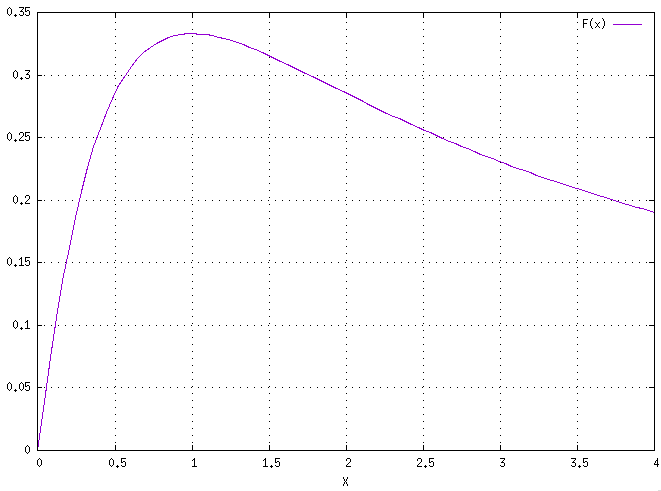
\includegraphics[width=0.5\textwidth]{f.png}
\end{center}
This means that for $X\ll 1$, or $C_0\ll\dfrac{1}{u_7}$, an increase in concentration will decrease the initial ratio, which is never the case when dealing with
the 1-layer expression stated in equation \eqref{eq:level1}.

\end{document}

